\documentclass{beamer}
\usepackage[utf8]{inputenc}
\usepackage[T1]{fontenc}
\usepackage{lmodern}
\usepackage[english]{babel}
\usepackage{lsfolien}
\usepackage{hyperref}

\myfootline{System Modelling and Semantic Web}{Carsten Lehmann}

\title{Problem Solving Tools - Trimming
	\vskip1em}

\subtitle{Module System Modelling and Semantic Web}

\author{Carsten Lehmann}

\date{June 21 2022}


\begin{document}

	\begin{frame}[plain]
		\maketitle
	\end{frame}

	\section{Topic overview}
	
	\begin{frame}{What is Trimming?}
		\begin{columns}
			\column{.4\textwidth}
			\begin{itemize}
				\item The change in the automotive industry from dealers to direct sales
				\item Lean Management 
				\item System on a chip
			\end{itemize}
			\column{.6\textwidth}
			\begin{figure}
				\centering
			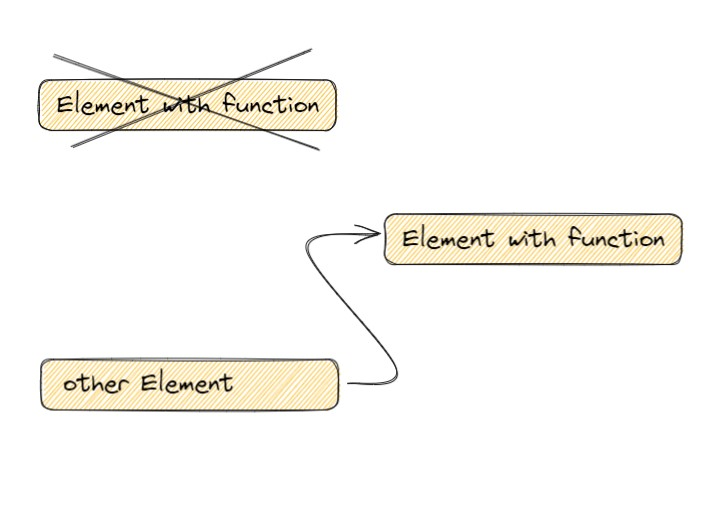
\includegraphics[width=.7\textwidth]{img/Intro.jpg}
				\caption{Trimming Principle}
			\end{figure}	
		\end{columns}
		Many processes and products follow the trend of trimming. Often to save costs while maintaining the same function.
	\end{frame}
	
	\begin{frame}{Def. of Trimming}
		The problem-solving tool trimming attempts to simplify a system in such a way that the same or better function is provided, but elements of the system can be removed.
	\end{frame}
	
	\begin{frame}{Brief overview of contents}
		\begin{itemize}
			\item Basic rules of the Trimming tool and system improvements
			\item Prerequisites for trimming usage
			\item Case studiy
		\end{itemize}
	\end{frame}
	
	\begin{frame}{Content Details}
		\begin{itemize}
			\item Basic rules of the Trimming tool and system improvements
    		\begin{itemize}
    			\item for physical Elements in a system
    			\item for processes
    		\end{itemize}
			\item Prerequisites for trimming application
    		\begin{itemize}
    			\item function capture
    			\item viable system tests
    			\item managing situations where elements are functionally coupled
    		\end{itemize}
			\item Case studies for systems:
    		\begin{itemize}
    			\item Example of Trimming on a Product
    		\end{itemize}
		\end{itemize}
	\end{frame}
	
	\section{Basic rules of the Trimming tool and system improvements}
	
	\begin{frame}{The Trimming Tool}
	The system have to be very well known before trimming \\
	Main goal of trimming: to remove unnecessary elements from a system
		\begin{itemize}
			\item Why don’t we eliminate this element?
			\begin{itemize}
    			\item Do we need the useful function(s) performed by this element?
    			\item Can one of the other elements in the system perform the useful function(s) instead?
    			\item Could we modify one of the other elements to perform the useful function(s)?
    			\item Is there an element or resource around the system that can perform the function(s)?
    			\item Is there an element or resource around the system that could be modified to perform the function?
    			\item Can we perform the function(s) by combining other elements and resources?
		    \end{itemize}
		\end{itemize}
	\end{frame}
	
	
	\begin{frame}{The Trimming Tool}
		\begin{block}{Why don’t we eliminate this element?}
			The questions are examined from top to bottom. If questions can be answered positively further up, this usually leads to a more ideal solution.
		\end{block}
	\end{frame}
	
	
	\begin{frame}{Trimming Question 1/6}
		\begin{columns}
			\column{.6\textwidth}
		Do we need the useful function(s) performed by this element?
		\begin{itemize}
			\item Does the element have any useful function at all? (visible in the FAA)
			\item Determine whether the useful functions are actually required
			\item Element must not perform other useful tasks in the system
			\item Element must not affect functionality of the system in future scenarios
		\end{itemize}
			\column{.4\textwidth}
			\begin{figure}
				\centering
				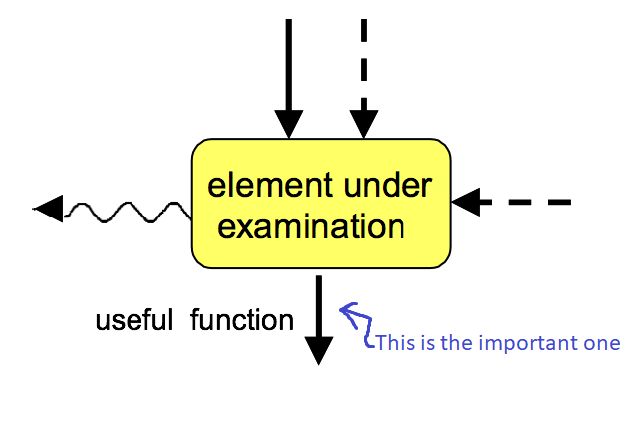
\includegraphics[width=1.1\textwidth]{img/q1.png}
				\caption{Useful Outgoing Functions Will Determine Whether the Element can be trimmed}
			\end{figure}	
		\end{columns}
	\end{frame}
	
	\begin{frame}{Trimming Question 2/6}
		Can One Of The Other Elements Perform The Function Instead?
		\begin{itemize}
			\item could other elements in the FAA model take over the function of the element we want to trim?
			\item Determine whether the useful functions are actually required
			\item Start with elements that are most closely connected to the trimmed part
			\item from there, work forward to elements in the model furthest from the element
		\end{itemize}
	\end{frame}
	
	
	\begin{frame}{Trimming Question 3/6}
		Could We Modify One Of The Other Elements To Perform The Useful Function(s)?
		\begin{itemize}
			\item Can we modify an element to perform the function?
			\item For this it is useful to analyze the evolutionary state of the respective elements.
			\item Start with elements that least evolved
			\item from there, work forward to elements with less evolutionary Potential
		\end{itemize}
		
		See next Page...
	\end{frame}
	
	\begin{frame}{Trimming Question 3/6}
	Could We Modify One Of The Other Elements To Perform The Useful Function(s)?
		\begin{figure}
			\centering
			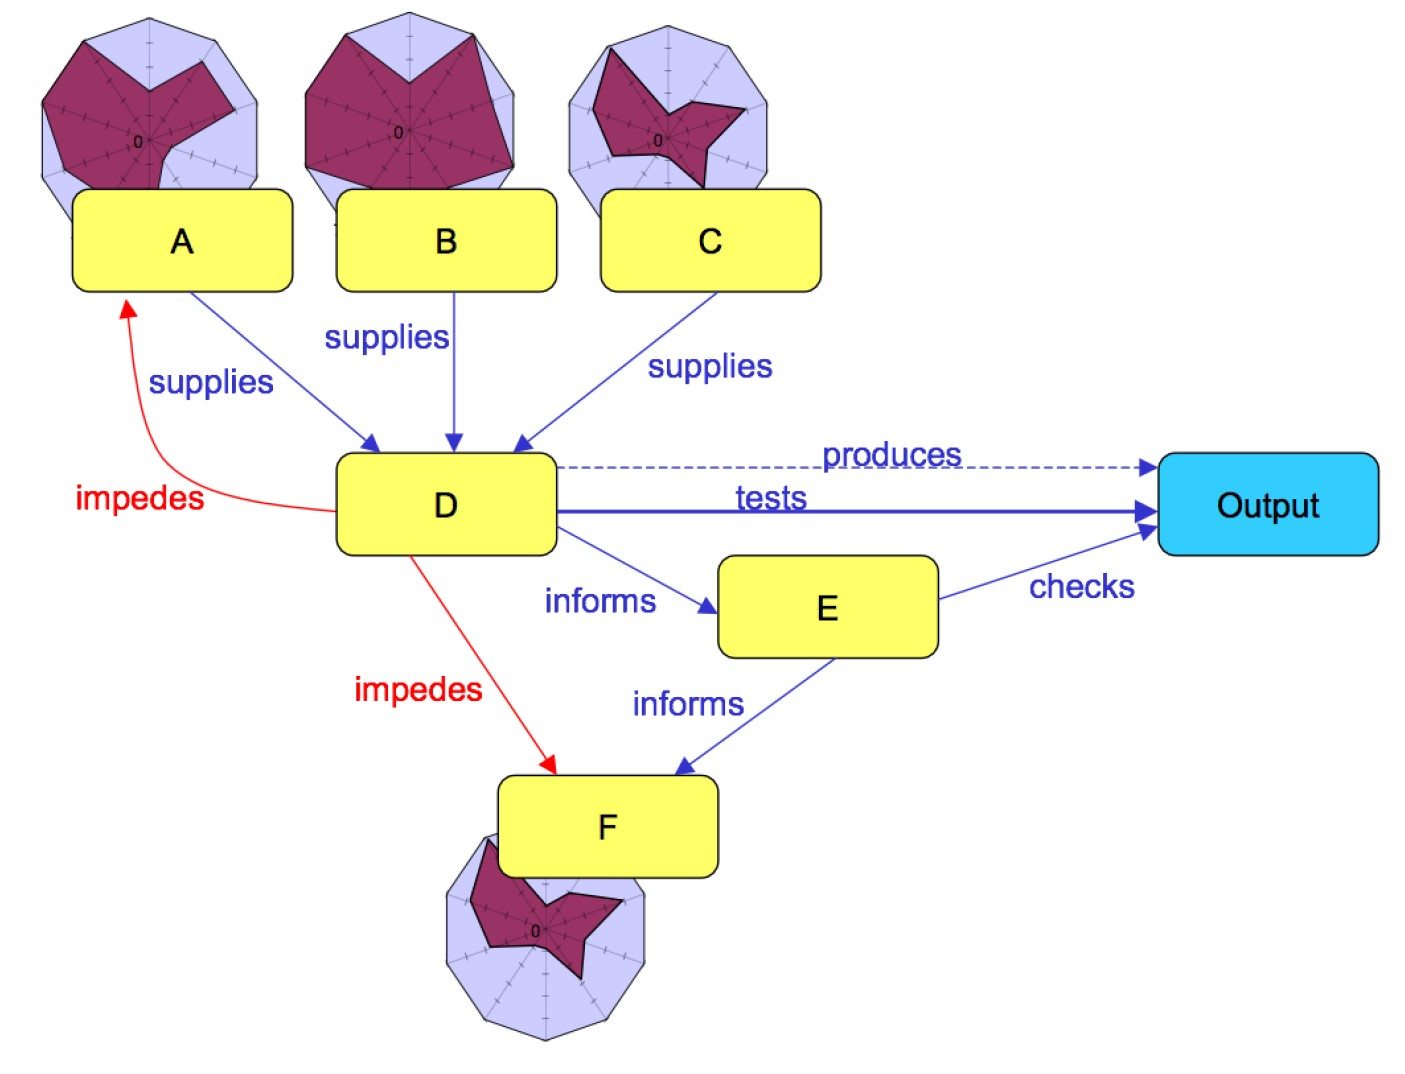
\includegraphics[width=0.6\textwidth]{img/q3.jpg}
			\caption{Evolution Potential Radar Plots For Elements In FAA Model}
		\end{figure}
	\end{frame}
	
	\begin{frame}{Trimming Question 4/6}
		Is There An Element Or Resource Around The System That Can Perform The Function(s)?
		\begin{itemize}
			\item look outside the system for resource that directly fulfills the function of the element
			\item Problem/Opportunity Explorer analysis -> is there an usable element in this list? 
			\item resource check-lists: more generally approach
			\item pay particular attention to the category of ‘low-cost resources’
		\end{itemize}
	\end{frame}
	
	
	\begin{frame}{Trimming Question 5/6}
		Is There An Element Or Resource Around The System That Could Be Modified To Perform The Function(s)?
		\begin{itemize}
			\item look at untapped evolutionary potential in elements or resources outside
			\item if a resource outside is evolved, could it perform the required action?
		\end{itemize}
	\end{frame}
	
	\begin{frame}{Trimming Question 6/6}
		Can I Perform The Function(s) By Combining Other Elements And Resources?
		\begin{itemize}
			\item combination between two or more existing elements
			\item combination between an existing element and one or more outside resources
			\item combination between two or more outside resources
		\end{itemize}
	\end{frame}
	

	\begin{frame}{Trimming for processes}
		Questions are essentially the same as above, just applied to processes.
		\begin{itemize}
			\item Do we need the useful function(s) performed by this process step?
			\item Can one of the other steps in the process perform the useful function(s) instead?
			\item Could we modify one of the other existing process steps to perform the useful function(s)?
			\item Can we introduce a new, simpler, process step that can perform the function(s)?
			\item Can we modify a process step from a different existing system to perform the function?
			\item Can we perform the function(s) by combining other process steps?
		\end{itemize}
	\end{frame}
	
	
	\section{Trimming Sequence}
	
	\begin{frame}{Trimming Sequence}
		Certain guidelines for application of trimming, but they do not tell us which elements can be trimmed in which order.\\
		Rules for this are not yet complete or generalizable, but there are four useful guidelines:
		\begin{itemize}
			\item elements with the highest number of not wanted functions connected to them are a prime candidate for trimming
			\item elements with the highest value offer the biggest trimming benefit
			\item highest elements in the functional hierarchy should be prioritized
			\item elements that deliver the smallest number of useful functions
		\end{itemize}
	\end{frame}
	
	\section{Trimming – The Bigger Picture}

	\begin{frame}{Trimming – The Bigger Picture}
		There are 3 aspects that are important to check if trimming should be used at all:
		\begin{itemize}
			\item[a)] function capture
            \item[b)] viable system tests
            \item[c)] managing situations where elements are functionally coupled
		\end{itemize}
	\end{frame}

	\begin{frame}{a) function capture}
		\begin{itemize}
			\item Record all functions present in a system as thoroughly and completely as possible
			\item FAA should be comprehensive and preferably validated by more than one person
			\item be absolutely sure that ALL useful function arrows are captured, pointing away from the element
		\end{itemize}
	\end{frame}

	\begin{frame}{b) viable system tests}
    	Viable System Model (VSM) according to Stafford Beer describes 5 necessary conditions for viability of a system:
		\begin{itemize}
			\item Implementation
			\item Co-ordination
			\item Intelligence
			\item Control
			\item Policy
		\end{itemize}
	\end{frame}
	
	\begin{frame}{b) viable system tests}
		\begin{block}{Implementation}
			defined as the parts of the system that are responsible for performing the main activities and can then be subdivided into subsystems, which are again considered viable system 
		\end{block}
		\begin{block}{Co-ordination}
			Individual elements and the system must communicate with each other. The more they do this and the less is imposed from above, the more autonomously the elements or subsystems function.
		\end{block}
	\end{frame}
	
	\begin{frame}{b) viable system tests}
		\begin{block}{Intelligence}
			Is the two-way linkage between the primary activity of the system and its environment. This enables adaptation to future, changing environmental influences.
		\end{block}
		\begin{block}{Control}
			Defined in VSM as the (two-way) communication between subunit and meta-level.
		\end{block}
		\begin{block}{Policy}
			The policy function provides closure to the system as a whole by deifying the overall direction, values, and purpose of the organizational unit.
		\end{block}
	\end{frame}
	
	
	\begin{frame}{b) viable system tests}
		Key point: If you try to remove one of these essential elements from a system, you basically have to find a replacement for them, because the system is not viable without them.
	\end{frame}
	
	\begin{frame}{c) Coupled Functional Requirements}
		The complexity of a system increases over time and is then also optimized more and more. The complexity of a system does not correspond to the number of elements. High complexity can also be generated by few elements with many functions.\\
		\vspace{\baselineskip}
		Trimming must never endanger autopoetic (self-sustaining) capability level of the system\\
		\vspace{\baselineskip}
		Important questions before trimming an element from the system:
		\begin{itemize}
			\item Are there any coupled functions?
			\item Are there aspects of the element to be pruned that link our system to the system at the next higher level in the hierarchy?
		\end{itemize}
		If the answer to either question is "yes," trimming should be used only with caution.
	\end{frame}
	
	
		
	\begin{frame}{Example}
		\begin{figure}
			\centering
			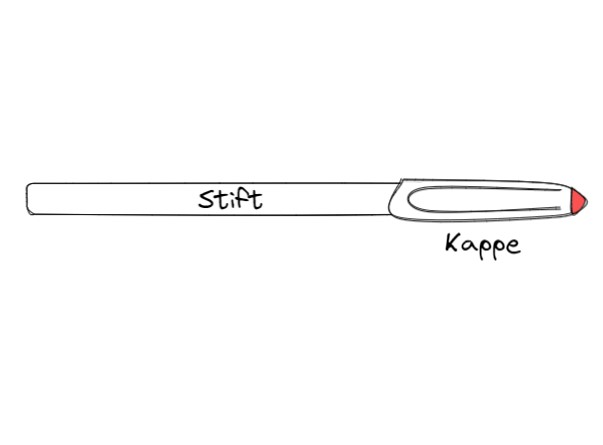
\includegraphics[width=0.6\textwidth]{img/ex.jpg}
			\caption{Example of Trimming on a Product   (www.michael-patra.de)}
		\end{figure}
	\end{frame}
	
	\begin{frame}{References}
		\begin{itemize}
			\item[1] Darell L. Mann. Hands-on systematic innovation for Business and Management. IFR Press, 2014
		\end{itemize}
	\end{frame}

\end{document}
